\section{Partikelschwarm-Algorithmus}

\subsection{Algorithmus}
Für die Partikelschwarm-Optimierung sind folgende Zustandsdaten zu jedem Partikel notwendig: \\
\begin{align*}
	x_i: & \text{aktuelle Position}\\
	v_i: & \text{aktuelle Geschwindigkeit}\\
	p_i: & \text{persönlich beste Position} \\
	l_i: & \text{beste Position des Schwarms}
\end{align*} \\

\subsubsection{Initialisierung}
Üblich ist die Initialisierung gemäss folgenden Formeln: \\
\begin{align}
	x_i(0) &= U(min,max) \\
	v_i(0) &= \frac{U(min,max) - x_i(0)}{2} \label{Vi-old} \\ 
	p_i(0) &= x_i(0)
\end{align} \\
Die Erfahrung hat gezeigt, dass mit der Initialisierung der Geschwindigkeit gemäss Gleichung \ref{Vi-old} die Partikel bei hohen Dimensionen den Suchraum praktisch unmittelbar verlassen. Um dies zu beheben wurde folgende angepasste Initialisierung eingeführt: \\
\begin{equation}
	v_i(0) = U(min - x_i(0), max - x_i(0))
\end{equation}

\subsubsection{Update der Geschwindigkeit}
Bei jeder Iteration werden die Zustandsdaten für jedes Partikel neu berechnet. Die neue Geschwindigkeit ist eine Linearkombination von drei Vektoren. Die Position wird gemäss Gleichung \ref{Pos-Update} aktualisiert. \\
\begin{align}
	v_{i}(t+1) &= \mathcal{C}(v_i(t),\, p_i(t)-x_i(t),\, l_i(t)-x_i(t)) \\
	x_{i}(t+1) &= x_i(t) + v_i(t+1) \label{Pos-Update}
\end{align}

Über die korrekte Wahl der Linearkombination $\mathcal{C}$ wurden bereits ganze Arbeiten geschrieben. Weit verbreitet, wenn auch nicht ideal ist die Berechnung gemäss Gleichung \ref{Vel-Update}. \\
\begin{equation}
	v_i(t+1) = w v_i(t) + U(0,c_1) (p_i(t)-x_i(t)) + U(0,c_2) (l_i(t)-x_i(t))\label{Vel-Update}
\end{equation}

mit den folgenden Parametern:
\begin{align*}
	w &: \text{Intertia Weight} \\
	c_1 &: \text{Cognitive Factor} \\
	c_2 &: \text{Social Factor}
\end{align*}
Diese Parameter, auch Acceleration Coefficients genannt, beeinflussen das  Verhalten und die Konvergenz des Schwarms. Hohe $c_1$ und $c_2$ führen zu abrupteren Bewegungen und höheren Beschleunigungen. Mit der Gewichtung dieser beiden Faktoren lässt sich weiter einstellen, wie stark sich die Partikel von Schwarm beeinflussen lassen. Wie genau diese Parameter eingestellt werden ist von der Problemstellung abhängig. Gemäss \cite{Clerc-Stagnation} haben sich folgende Werte für einfache Probleme als zweckmässig erwiesen:
\begin{equation}
	\left\lbrace \begin{array}{lllll}
		w & = & \frac{1}{2 \ln(2)} & \simeq & 0.721 \\
		c_1 = c_2 & = & \frac{1}{2} + \ln(2) & \simeq & 1.139 \\
	\end{array}	\right. 
\end{equation} \\


Die Herleitung der neuen Geschwindigkeit wird in Abbildung \ref{Fig-Visualisierung-Geschwindigkeit} visualisiert. Die Punkte $x'_i$ und $x''_i$ werden zufällig aus den zu den Achsen parallelen, gelb bzw. grün hinterlegten Bereichen generiert.  \\
\begin{figure}[htbp]
	\centering
	\documentclass{standalone}

\usepackage{tikz}
\usetikzlibrary{arrows,decorations.pathmorphing,positioning,fit,petri}
\usetikzlibrary{calc,intersections,through,backgrounds,graphs}
\usetikzlibrary{patterns,decorations.pathreplacing}

\begin{document}

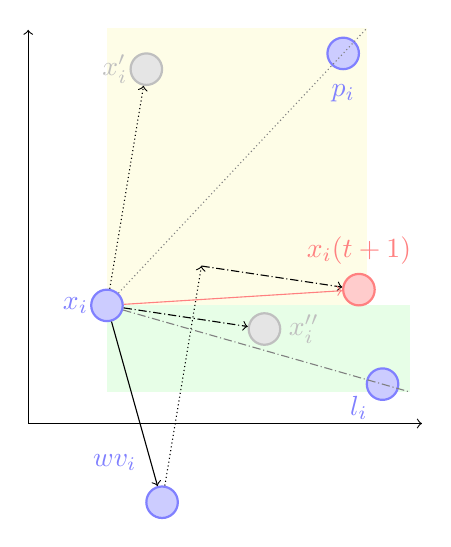
\begin{tikzpicture}
	% Styles
	[
	point/.style={circle,draw=blue!50,fill=blue!20,thick, inner sep=0pt,minimum size=4mm},
	vpoint/.style={circle,draw=gray!50,fill=gray!20,thick, inner sep=0pt,minimum size=4mm},
	endpoint/.style={circle,draw=red!50,fill=red!20,thick, inner sep=0pt,minimum size=4mm},
	]
                      
	% Axis
	\draw[->] (0,0) -- (5,0);
  	\draw[->] (0,0) -- (0,5);
	
	% Shaded Parts
	\fill[gray!10!yellow!10] (1,1.5) rectangle (4.3,5.02);
	\fill[gray!10!green!10] (1,1.5) rectangle (4.85,0.4);

	% Nodes
	\node at (1.5,4.5)	(xi1)	[vpoint]	{};
	\node at (3,1.2)	(xi2)	[vpoint]	{};
	\node at (4,4.7)	(pi)	[point] 	{};
	\node at (4.5,0.5)	(li)	[point] 	{};
	\node at (1.7,-1)	(wvi) [point]	{};
	\node at (1,1.5)	(xi)	[point]	{} 
		edge [->,densely dotted]			(xi1)
		edge[densely dotted,gray]		(4.3,5.02)
		edge[->,densely dashdotted]		(xi2)
		edge[densely dashdotted,gray]	(4.85,0.4);
	\node at (4.2,1.7)	(xit)	[endpoint] {};
	\draw[->] (xi) -- (wvi);
	\draw[->,densely dotted] (wvi)  -- (2.2,2);
	\draw[->,densely dashdotted] (2.2,2) -- (xit);
	\draw[->,red!50]	(xi) -- (xit);

	% Text
	\node[blue!50]		at (0.6,1.5)	{$x_i$};
	\node[gray!50]		at (1.1,4.5) 	{$x'_i$};
	\node[gray!50]		at (3.5,1.2) 	{$x''_i$};
	\node[blue!50]		at (4,4.2)		{$p_i$};
	\node[blue!50]		at (4.2,0.2)	{$l_i$};
	\node[red!50]		at (4.2,2.2)	{$x_i(t+1)$};
	\node[blue!50]		at (1.1,-0.5)	{$wv_i$};

\end{tikzpicture}

\end{document}
	\caption{Visualisierung der Geschwindigkeit}
	\label{Fig-Visualisierung-Geschwindigkeit}
\end{figure}


\subsection{Grösse des Schwarms}
Über die ideale Grösse des Partikelschwarms lassen sich keine exakten Angaben machen. Gemäss \cite{Clerc-Standards} lässt sich die Grösse $S$ des Schwarms in Abhängigkeit der Dimension $D$ wie folgt ausdrücken:
\begin{equation}
	S = 10 + \left[ 2 \cdot \sqrt{D} \right]
\end{equation}
Die Näherung führt jedoch oft zu ungeeigneten Werten, weshalb Maurice Clerc vorschlägt, einen beliebigen Wert um $40$ zu wählen. Die theoretischen Grundlagen zur idealen Grösse des Schwarms sind nicht bekannt.


\subsection{Exploration-Exploitation Tradeoff}
Der Exploration-Exploitation Tradeoff sagt aus, dass ein Partikelschwarm nicht gleichzeitig ein möglichst grosses Zielgebiet absuchen kann (Exploration) und einen Bereich so genau wie möglich durchsuchen kann (Exploitation). Dieses Verhältnis von Exploration zu Exploitation hat einen starken Einfluss auf die Konvergenz. Generell kann gesagt werden, dass je höher die Inertia Weight $w$, desto weniger verlangsamt sich die Geschwindigkeit der Partikel, weshalb die Exploration stärker gewichtet ist.

\subsection{Parallelisierung}
Aus der Beschreibung des Algorithmus wird schnell ersichtlich, dass die Partikelschwarm-Optimierung sehr gut für eine parallelisierte Berechnung geeignet ist. Die Aktualisierung der Geschwindigkeit und Position kann für alle Partikel gleichzeitig, parallel erfolgen. Bei rechenintensiven Problemen ist dies ein enormer Vorteil gegenüber anderen Optimierungsmethoden.